\documentclass[onecolumn, draftclsnofoot,10pt, compsoc]{IEEEtran}
\usepackage{graphicx}
\usepackage{url}
\usepackage{setspace}
\usepackage[parfill]{parskip}
\usepackage{geometry}
\geometry{textheight=9.5in, textwidth=7in}
\usepackage[pdf]{pstricks}
\usepackage{pst-gantt}

% 1. Fill in these details
\def \CapstoneTeamName{Aggregators}
\def \CapstoneTeamNumber{71}
\def \GroupMemberOne{Carter Olsen}
\def \GroupMemberTwo{Megan Liles}
\def \GroupMemberThree{Aalok Borkar}
\def \GroupMemberFour{Race Stewart}
\def \CapstoneProjectName{News Aggregator Web Development}
% \def \CapstoneSponsorCompany{	Cheap Robots, Inc}
\def \CapstoneSponsorPerson{Joseph Louis}

% 2. Uncomment the appropriate line below so that the document type works
\def \DocType{		%Problem Statement
				%Requirements Document
				%Technology Review
				Design Document
				%Progress Report
				}
			
\newcommand{\NameSigPair}[1]{\par
\makebox[2.75in][r]{#1} \hfill 	\makebox[3.25in]{\makebox[2.25in]{\hrulefill} \hfill		\makebox[.75in]{\hrulefill}}
\par\vspace{-12pt} \textit{\tiny\noindent
\makebox[2.75in]{} \hfill		\makebox[3.25in]{\makebox[2.25in][r]{Signature} \hfill	\makebox[.75in][r]{Date}}}}
% 3. If the document is not to be signed, uncomment the RENEWcommand below
% \renewcommand{\NameSigPair}[1]{#1}

%%%%%%%%%%%%%%%%%%%%%%%%%%%%%%%%%%%%%%%
\begin{document}
\begin{titlepage}
    \pagenumbering{gobble}
    \begin{singlespace}
    	
\includegraphics[height=4cm]{coe_v_spot1}
        \hfill 
        % 4. If you have a logo, use this includegraphics command to put it on the coversheet.
        %\includegraphics[height=4cm]{CompanyLogo}   
        \par\vspace{.2in}
        \centering
        \scshape{
            \huge CS Capstone \DocType \par
            {\large\today}\par
            \vspace{.5in}
            \textbf{\Huge\CapstoneProjectName}\par
            \vfill
            {\large Prepared for}\par
            % \Huge \CapstoneSponsorCompany\par
            \vspace{5pt}
            {\Large\CapstoneSponsorPerson\par}
            {\large Prepared by }\par
            Group \CapstoneTeamNumber\par
            % 5. comment out the line below this one if you do not wish to name your team
            \CapstoneTeamName\par 
            \vspace{5pt}
            {\Large
                \GroupMemberOne\par
                \GroupMemberTwo\par
                \GroupMemberThree\par
                \GroupMemberFour\par
            }
            \vspace{20pt}
        }
        \begin{abstract}
        % 6. Fill in your abstract    
            This document describes the design components of the News Aggregator website. It is structured as follows. A brief overview section will outline the purpose, intended audience, definitions, and project context. This is followed by the body of the document which further details the design of the project. The design description defines the stakeholders, views and viewpoints defined in the IEEE 1016 format. The project was broken up into four components: the front end, the back end, the natural language processing model, accessibility, database management, scraping of RSS feeds and mobile-friendliness. Each of these sections are discussed in depth in terms of design description.

        \end{abstract}     
    \end{singlespace}
\end{titlepage}
\newpage
\pagenumbering{arabic}
\tableofcontents
% 7. uncomment this (if applicable). Consider adding a page break.
%\listoffigures
%\listoftables
\clearpage
\section{Introduction}
\subsection{Scope}
This document covers the design choices in detail for each section of our project. It also covers different viewpoints of the design and how we will approach them and the concerns that come with them.
\subsection{Purpose}
The main goal of the News Aggregator web tool is to dissolve journalistic echo-chambers, and give users a less biased view into the events happening around them. This document exists both for development of the project and to provide a detailed description of the design plans.
\subsection{Summary}
News Aggregator will take the form of a multi-layered web application, consisting of a Node.js back end server, a React front end interface, a Python based aggregator script and natural language processing model, and finally a MongoDB data store to hold all scraped and processed news articles.
\section{References}
\begingroup
\renewcommand{\addcontentsline}[3]{}% Remove functionality of \addcontentsline
\renewcommand{\section}[2]{}% Remove functionality of \section
\bibliographystyle{IEEEtran}
\bibliography{sources}
\endgroup

\section{Glossary}
\begin{itemize}
    \item Code Module: An independent and interchangeable, unit of code.
    \item Corpus: A collection of words.
    \item GenSim: A topic modeling and natural language processing library.
    \item Lemmatize: Sort words by grouping inflected or variant forms of the same word.
    \item Middleware: Code that acts as a bridge between pieces of an application.
    \item RSS Feed: A web feed allowing applications to access updates to websites in a standardized, computer-readable format.
    \item TF-IDF: Term Frequency - Inverse Document Frequency
    \item Tokenize: Break (text) into individual linguistic units.
\end{itemize}
\section{Design Description}
\subsection{Design Stakeholders}
\subsubsection{Joseph Louis}
Joseph Louis, an assistant professor in the Civil Engineering department, is the projects client. Joseph created the idea for the News Aggregator web application and consistently provides the team with feature requirements and stretch goals that he desires for the product.
\subsection{Design Viewpoints}
\subsubsection{Context Viewpoint}
Our context viewpoint reveals the functionalities between the user and the system. The main functionalities in this project are the user functionalities, the web application functionalities and the RSS scraper functionalities. The user's viewpoint should not notice the system functionalities. To the user, they should be given an interface that is intuitive and easy to navigate so they don't have to think about what is going on behind the scenes. The context viewpoint diagram is shown in Figure \ref{context_vp}.
\begin{figure}[!ht]
    \centering
    \caption{Context Viewpoint Diagram}
    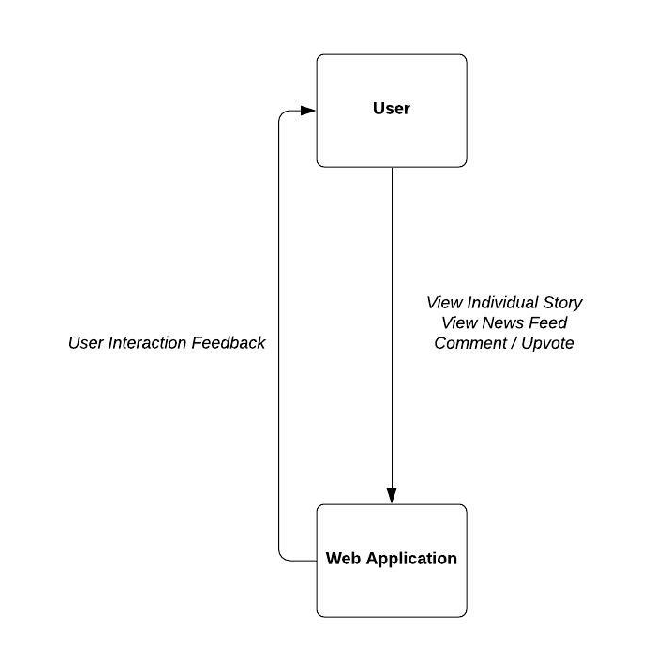
\includegraphics[width=0.4\textwidth]{context_vp.eps}
    \label{context_vp}
\end{figure}

\hangindent=0.5cm \textbf{Design Concern}: The main concern of this context is making sure that user is given an interface that is easy to use. This includes an accessible, intuitive design presenting accurately grouped news stories.

\hangindent=0.5cm \textbf{Analytical Methods}: To design this interface, we will use Bootstrap, which is the most popular library for using modern design in your web application. We will also use user testing to ensure that our design is accepted by users. 

\hangindent=0.5cm \textbf{Rationale}: This viewpoint was included because we have many parts to our application and it is important to understand how they all work together to make a functional web application.

\subsubsection{Composition Viewpoint}
Our project will be split into the following sections:
\begin{itemize}
    \item User Interface Design and Components
    \item Web Server Design
    \item Database Structure and Design
    \item RSS Scraper Design
\end{itemize}
These sections will each be talked about in more detail in a later section. For this section, we will discuss the relationships between each component and how they are strung together. Figure \ref{composition_vp} gives a diagram on our project design.

\begin{figure}[!ht]
    \centering
    \caption{Composition Viewpoint Diagram}
    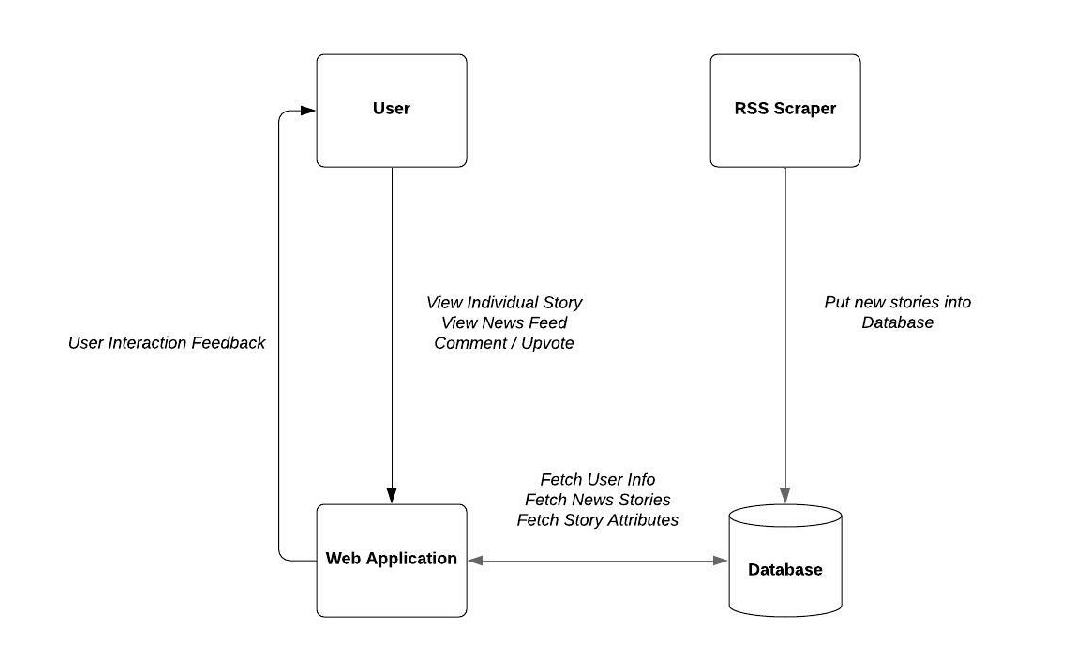
\includegraphics[width=0.6\textwidth]{composition_vp.eps}
    \label{composition_vp}
\end{figure}

\hangindent=0.5cm \textbf{Design Concern}: The way we compose our project affects the performance, ease of future development and how easy it is to implement our design now. This viewpoint is important because if this project is ever transferred to anyone else, a well-designed composition will lead to a quicker and easier knowledge transfer.

\hangindent=0.5cm \textbf{Analytical Methods}: We can analyze the success of our design by how easily we can transfer knowledge between group members in this project. This one is hard to analyze because the only people involved in the composition are the group members of this project.

\hangindent=0.5cm \textbf{Rationale}: This viewpoint was included because the design of this project plays an important role in knowledge transfer, performance and componentization of elements in our project. The front-end of the web application relies on data that the back-end retrieves from the database. The database gets its data from the RSS scraper. As you can see, these elements of the project can all be separated into components that rely on each other, but work individually from each other.

\subsubsection{Interface Viewpoint}
The Interface viewpoint provides information designers, programmers, and testers the means to know how
to correctly use the services provided by a design subject. With our site, there will be a few different interfaces that our programmers will need to interact with, and in the long term users will need to interact with the interface that will make up the website as well. The purpose of this viewpoint is to clarify how these interfaces will mesh to form a neat, intuitive final product.

\hangindent=0.5cm \textbf{Design Concern}:
The view with the most interest in this viewpoint will be the developers, since the sponsor, Joseph Louis, doesn't necessarily concern himself with the technical aspect of the project as long as it meets his wishes. The main external interfaces are going to be some user's computer or mobile device and the external monitors or screens that are used to display the site. The internal interfaces of the project are going to be whatever browser a user might use, whatever database is used to store information, and whatever development tool the programmers choose to use in the development of the site. Short term, developers are very concerned with the interface viewpoint, but long term, users will certainly be impacted by it. 

\hangindent=0.5cm \textbf{Analytical Methods}: This viewpoint is going to encourage the creation of a site that will function smoothly and work for anyone who wishes to access it. The interfaces that the developers use and the interfaces that users will interact with during their experience are critical in this goal. This viewpoint is therefore going to provide an understanding for what needs to be done in terms of creating and interacting with smooth and simple interfaces. The assessing process of these interfaces with include an accessibility score using https://wave.webaim.org/.

\hangindent=0.5cm \textbf{Rationale}: This viewpoint was included because there are multiple different technologies used in the process of creating this site and the interfaces that the users are going to be interacting with. This means that those with technical interests in the project, namely the developers, will be affected greatly by the way those interfaces interact. 

\subsubsection{Algorithm Viewpoint}
The algorithm viewpoint for this project will cover our choice in the algorithm to match articles together. In GenSim, a popular natural language processing library in Python, they provide tools to perform similarity analysis on documents that you provide it. We are choosing to use the TF-IDF scores to match up documents, as this seems to be the most accurate for our case. The TF-IDF score for a term is defined as the term frequency of a term * the inverse frequency that it appears in all of the documents. This is useful for matching up documents that have unique keywords in them.

\hangindent=0.5cm \textbf{Design Concern}: The major concern of this algorithm is how accurate it is. We need a high accuracy rate, so we don't pair two articles that are talking about different topics. This would defeat the purpose of our web application.

\hangindent=0.5cm \textbf{Analytical Methods}: We can analyze the accuracy of the model by manually comparing the stories that it matches to and seeing if they really are talking about the same topic. There are also ways to automate this by creating a test set of our data and manually grouping them and testing against that grouping. Both of these methods will involve some manual testing.

\hangindent=0.5cm \textbf{Rationale}: The reason we chose this viewpoint is because the algorithm we use is a key factor in how accurate our grouping of similar articles is. This is a key part of our web site and we need to make sure that this has high accuracy rates.

\section{Approach}
\subsection{Back-end of Web Application}
For the News Aggregator application to function, it will need a back end to not only host the front end, but to also provide the main functionality of sending and updating the news articles present on said front end.
\subsubsection{Concerns}
One of the biggest concerns in regards to the back-end is that of latency issues and errors in data being sent to the front end through API's. To ensure that there are no issues on this front, and that all pieces of the application stack are able to function in harmony, a JavaScript (Node.js) server will be created to support the JavaScript (React) front end, ensuring maximum synergy and performance safety,
\subsubsection{Approach}
Because the News Aggregator application will rely primarily on client-side rendering to produce content for users, the Node.js server will utilize the Express web application framework, and take the form of an express application. First and foremost, this application will include middleware routing to both host and ensure that content is re-rendered whenever a user navigates to another page. Along with the web-hosting responsibilities, this server application will maintain a direct connection with the MongoDB data store, and provide an active API for the client side to receive newly aggregated news story clusters from the data store. The server will also maintain listeners to actively recognize updates within the MongoDB data store and ultimately use its API to alert the front end to update. Although relatively succinct in nature, this back-end server plays a crucial role in hosting, updating, and empowering the News Aggregator web application as a whole.
\subsection{Front-end of Web Application}
\subsubsection{Concerns}
The most important concern for the design of the Front-end of the Web Application is to make the website intuitive to use. If the application is too complex, difficult to learn and remember how to use, users will be turned away from using it. Our application must have a critical balance between a simple user interface and an intriguing user experience.

\subsubsection{Approach}
Our approach to designing the front-end will involve several steps which involves an intuitive user interface, social media sharing, and an inviting user experience. 

\hangindent=0.5cm \textbf{User Interface}:
This concern of an intuitive user interface involves several steps. The first step to achieve this goal is to design multiple personas to represent the population of users the application is targeting. The persona will target users who have a desire for reading news but may also include users who are not proficient using technology. The new site will include pop-up bubbles to highlight features on the website that most news websites do not include. This will help with the intuitive concept. The front-end design will also require mock-ups to help communicate what ideas the developers have to the client. Users studies will also be included as a step in designing the front-end to receive feedback about usability of the site and to learn how the developers can make it more intuitive. The last part of creating an intuitive user interface will be to use intuitive front-end features provided by Bootstrap. Bootstrap is known for it’s responsive front-end allowing user’s to understand how to use the web application thus working towards our goal of an intuitive web application.

\hangindent=0.5cm \textbf{Social Media Sharing}:
Social media sharing is another feature we will include in the design of the front-end of the application. This is an important feature on the website as it makes the user experience fun, competitive and intriguing. Social media sharing can drive usage of the site and increase visits allowing us to expand our population of target users. Social media buttons will be incorporated at the bottom of each news story allowing users to share the news post to popular social media platforms such as Twitter, Facebook and Reddit. This is an important aspect of the front-end as it will increase popularity of th web application and make the site interactive for users.

\hangindent=0.5cm \textbf{User Experience}:
The user experience will be approached once again with user studies allowing users to share their thoughts about using the web application and receiving feedback help the developers implement a better user experience. Another feature that will be incorporated to make the user experience better will be the ability for users to comment and like news stories. This allows users to interact with the site under their profile. Research will also be done to look at popular web applications and ways in which the user experience is heightened through the design of the front-end. 


\subsection{Natural Language Processing Model}
To accurately clusters new articles from various sources based off of their respective topics, a natural language processing model will run within the aggregator script. Beyond just classifying the articles fed into it, this natural language processing model will also have the responsibility of pre-processing the data it receives as input, as well as providing a properly shaped output for the aggregator script to then store within the MongoDB data store.
\subsubsection{Concerns}
The most concerning aspect of the natural language processing model is in regards to it's accuracy, as the entire functionality of the News Aggregator relies on the model's ability to correctly cluster news stories based off of their analyzed topics.
\subsubsection{Approach}
 The natural language processing model itself will be housed within a module of code responsible for pre-processing and outputting data, within the aggregator script. In more detail, the model’s module will begin with a section for extracting the tokenized root words and lemmatized data from the testing document csv files. The module will then have a section for accessing and initializing its dictionary and corpus using this collected data through the GenSim library, for processing and analyzing the text input it receives. The module will then construct and train the primary model, in this case what is known as a TF-IDF model, based off of the dictionary and corpus it constructed. After creating the actual model used for the classification of the articles, the module will then have a section specifically meant for processing new data fed in from the aggregator script, where it will then output a similarity score from zero to positive one, denoting the input articles closeness to an existing political topic in the database. After inputting this newly fed document back into the dictionary and corpus to enhance the accuracy of the TFIDF model, if the closeness score is below the threshold of 0.4, the module will have the task of inserting this input document as well as it’s new topic into the database for future articles to be compared to. Because of the modules structure, this process of categorizing articles and retraining the natural language processing model will continue perpetually as the aggregator script continues to pull in new articles from its connected RSS feeds.
\subsection{Accessibility}
With a modern website such as News Aggregator it is extremely important that the user experience is inclusive, and these guidelines ensure that all users, regardless of circumstance, will be able to utilize all of the website’s features without issue.
\subsubsection{Concerns}
Although creating the user interface components from scratch would guarantee that they fit the aesthetic profile that was originally intended, doing so might inadvertently run the risk of violating the Web Content Accessibility Guidelines (WCAG), and ultimately make the website less accessible. For this reason only WCAG compliant modules and button layouts from the Bootstrap CSS library will be used for the News Aggregator user interface. 
\subsubsection{Approach}
Starting from the physical top of the front end’s user interface, the interactive elements within the search bar of the site will have descriptive CSS values and associated text labels, and any of the banner images that do not actually convey article based contact, or are primarily decorative in nature, will be given a null alt text ‘(alt=””)’. Moving further down the UI and into the actual content grids, many of the buttons and instructional modules (if help button is clicked) will not rely solely on the appearance or shape of the button, instead opting to include several unique identifiers such as color and special icons to inform users of operations and actions regardless of device or visual circumstance. Within the grids of content displaying the articles, the blocks of text summarizing the documents that are over one sentence in length will be no longer than 80 characters in width, will have adequate line spacing, and will not require side scrolling if the page is expanded, as to ensure full inclusiveness when looking at article content. Along with maintaining inclusiveness through the content’s text, when displaying images that pertain to individual articles, any supporting text will be kept disjoint from the image itself, to ensure that the image is solely for aesthetic reasons and users have the ability to still distinguish the individual articles being displayed to them. Lastly, within the content grids, all links directing users to source articles will be explicit in their purpose, and will be distinguishable not only through color but also through underlining and bolding (increased text density) to ensure that every user will have the same understanding and access to the same content.
\subsection{Database Management}
Storing the news stories and the data associated with them is an essential for our project. For example, we need to store these stories because we need to info on what other stories they are related to, what keywords they have and other various attributes such as date published. For Database Management, we chose to go with MongoDB because of the cost, performance, and the document-style format for storing data fit with our use.
\subsubsection{Concerns}
One of the main concerns with any database management is security. We must ensure that we are storing users' emails and passwords securely for when we implement account creation. We also need to make sure that our queries on the data are efficient so we can get the data to the user in an efficient manner. Luckily, with a NoSQL database like MongoDB, they handle most of the querying, so we don't have to worry about making sure the queries are the most efficient they can be.
\subsubsection{Approach}
There are two parts of this approach that are important and they are storing data and querying for data.

\hangindent=0.5cm \textbf{Storing Data}: When storing data, it is important that we avoid duplicate entries of the same news story. That is why we have implemented an "article\_id" associated with each article that is unique to each story. Thanks to MongoDB's upsert feature, we can perform an insert query into the database where if the article ID already exists, it updates the information for the document, otherwise it inserts the new article into the database \cite{mongo_upsert}. 

\hangindent=0.5cm \textbf{Querying Data}: On the topic of querying data, it is important to make sure that you provide access control to the database. Because the application is open to the public, we must make sure that we have a read-only account that is secure and only being used by our back-end. We also want to make sure that our data isn't being overly queried. This can be done with caching and limiting of results sent in the response.

\subsection{Scraping of RSS feeds}
The scraping of each RSS feed involves downloading the feed's XML and parsing it.
\subsubsection{Concerns}
We need to make sure that this scraping of RSS feeds runs on a scheduled timer and that it doesn't insert duplicate data into the database. As discussed above, MongoDB handles the duplicate data by allowing us to use the upsert feature. As far as scheduling the scraping of data, it should run on an hourly basis, pulling new stories and parsing them to match them up with other similar stories.
\subsubsection{Approach}
There are many parts to making sure that our database is managed well. First, we need to make sure that we have created multiple accounts for various access levels. Second, we need to make sure that the naming of our tables and databases are consistent. Lastly, it is very important that we secure and encrypt any sensitive information from our users in the database. We will follow the best practices for securing sensitive data in MongoDB. To ensure that we are following the best practices, we will follow the Securing MongoDB Documentation that MongoDB provides \cite{secure_mongo}.

\subsection{Mobile-friendliness}
The process of ensuring that the site is mobile friendly includes coding the site in a responsive fashion, including the viewport meta tag, and repeated testing of the site on multiple devices.
\subsubsection{Concerns}
We need to make sure that the site functions as intended on any device, no matter the screen size. This could be difficult, depending much on how difficult we make it. For example, writing code for the front end in a responsive way requires having different pages of styling depending on the device that's viewing the site, but how can we be certain the type of device that's accessing it? What's the simplest way to go about this, given that we need to have so many different accommodations for devices of different sizes?
\subsubsection{Approach}
There are a few different components to keep in mind when making sure that the site is designed in a mobile-friendly fashion. Firstly, we need to make sure that we are able to display the site properly depending on the type of device that's accessing it. This includes the text and button size, the layout on the screen, and inclusion of the viewport meta tag so that the user doesn't have to scroll endlessly from side to side on a mobile device. Then, we need to make sure that we're able to test on a variety of devices. This is a must for developing a flexible, multi-platform front-end because we need to ensure that it will look great on any device.
\end{document}